% LaTeX snippets produced by plot-agent. Every numeric value traces to
% inputs/experimental_log.md; see figures/make_figures.py for the source
% lines.

\begin{figure}[htbp]
\centering
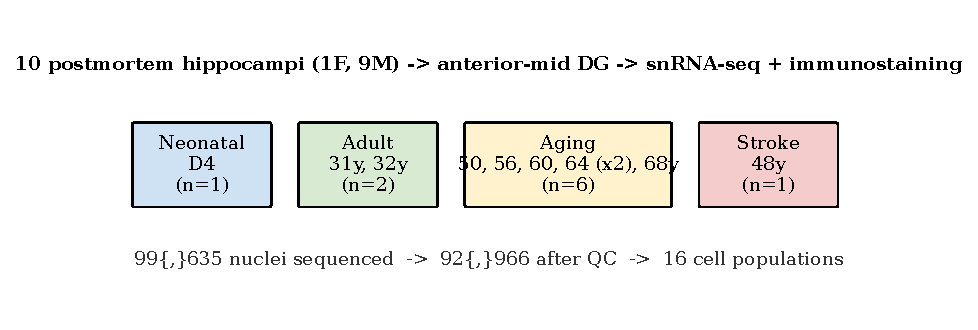
\includegraphics[width=0.95\textwidth]{figures/fig_donor_cohort.pdf}
\caption{Donor cohort and experimental design. Ten postmortem human hippocampi spanning neonatal (postnatal day 4, $n=1$), adult (31 and 32 years, $n=2$), aging (50, 56, 60, 64 (x2), 68 years, $n=6$), and stroke-induced injury (48 years, $n=1$) donors were dissected at the anterior-mid hippocampus containing the dentate gyrus, then processed by 10x Genomics single-nucleus RNA sequencing in parallel with paired immunostaining; 99{,}635 nuclei sequenced and 92{,}966 retained after QC, yielding 16 major cell populations.}
\label{fig:cohort}
\end{figure}

\begin{figure}[htbp]
\centering
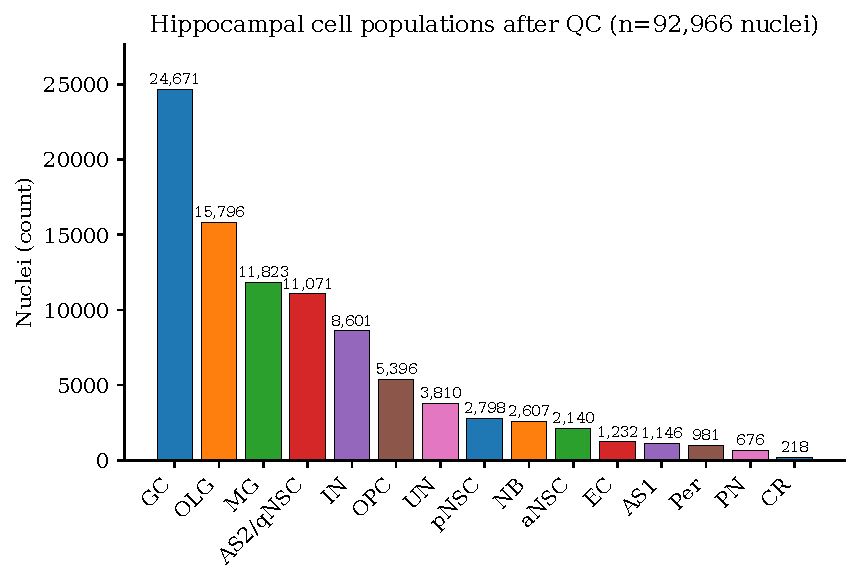
\includegraphics[width=0.95\textwidth]{figures/fig_cell_populations.pdf}
\caption{Nucleus counts per annotated cell population after quality control (total 92{,}966 nuclei). Granule cells (GC, 24{,}671) dominate, followed by oligodendrocytes (OLG, 15{,}796), microglia (MG, 11{,}823), astrocyte2/qNSC (AS2/qNSC, 11{,}071), and interneurons (IN, 8{,}601); the neurogenic progenitor fractions pNSC (2{,}798), aNSC (2{,}140), and neuroblast (NB, 2{,}607) are comparatively rare but resolvable.}
\label{fig:populations}
\end{figure}

\begin{figure}[htbp]
\centering
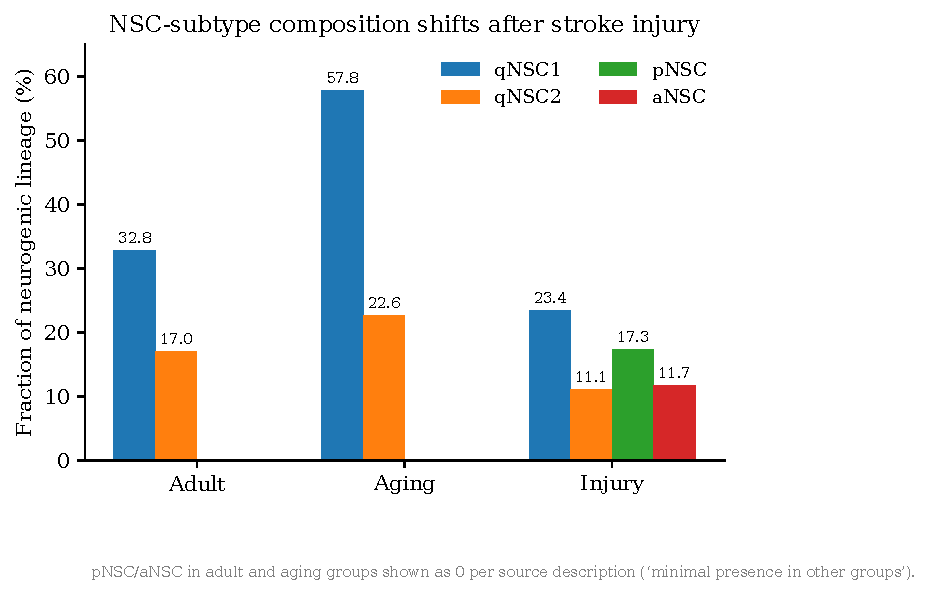
\includegraphics[width=0.82\textwidth]{figures/fig_lineage_fractions.pdf}
\caption{Stroke injury rebalances the neurogenic lineage toward primed and active NSC states. Within-lineage percentages of qNSC1, qNSC2, pNSC, and aNSC in adult, aging, and stroke-injured hippocampus, derived from the Figure 6D values in the experimental log. qNSC1 rises from 32.8\% in adult to 57.8\% in aging and then falls to 23.4\% after stroke, while pNSC and aNSC --- reported as ``minimal'' in adult and aging groups (shown as zero) --- recover to 17.3\% and 11.7\% respectively in the injured hippocampus.}
\label{fig:lineage}
\end{figure}

\begin{figure}[htbp]
\centering
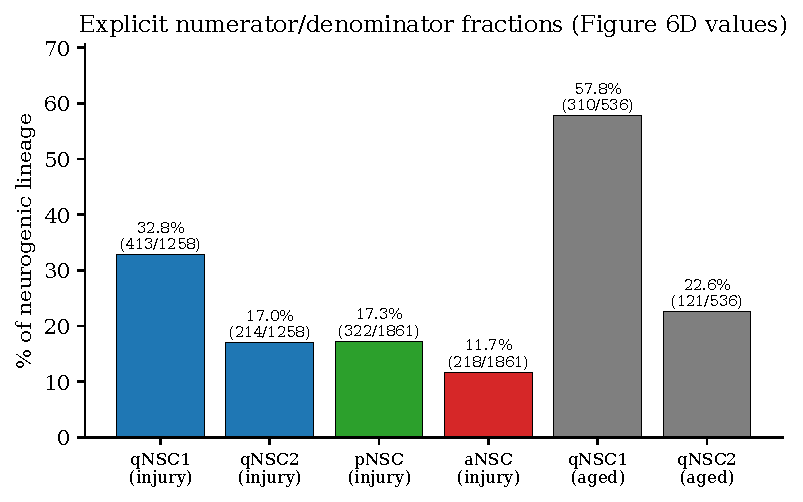
\includegraphics[width=0.92\textwidth]{figures/fig_injury_counts.pdf}
\caption{Absolute numerator / denominator counts underlying the neurogenic-lineage fractions. Stroke-injured counts (blue/green/red): qNSC1 413/1258 (23.4\%), qNSC2 214/1258 (11.1\%), pNSC 322/1861 (17.3\%), aNSC 218/1861 (11.7\%). Aged counts (grey): qNSC1 310/536 (57.8\%), qNSC2 121/536 (22.6\%). All values taken verbatim from the experimental log.}
\label{fig:injury_counts}
\end{figure}
